\documentclass[10pt,twocolumn,letterpaper]{article}
\usepackage{cvpr}
\usepackage[hyphens]{url}
\usepackage{times}
\usepackage{graphicx}
\usepackage{amsmath}
\usepackage{amssymb}
\usepackage[pagebackref=true,breaklinks=true,colorlinks,bookmarks=false]{hyperref}
\def\GroupID{G01} % <------- ENTER YOUR COMP 6321 group number here
\setlength{\parindent}{2em}
\setlength{\parskip}{0em}
\renewcommand{\baselinestretch}{1}

\begin{document}
\title{Is it Fake News? A Comparison of Traditional Machine Learning Models and Deep Learning Models for News Article Classification}
\author{Giselle Martel ID: 26352936 \and Firas Sawan ID: 26487815}
\maketitle
\begin{abstract}
\small
"Fake news" is a term which we hear more often in contemporary times, and "is part of a larger spectrum ranging from unintentional misinformation (e.g., sloppy reporting) to intentional disinformation (e.g., propaganda)"\cite{doi:https://doi.org/10.1002/9781118841570.iejs0128}. The spread of falsehoods and inaccuracies through social media and online news sources undermines societal progress \cite{doi:https://doi.org/10.1002/9781118841570.iejs0128}, and we estimate can spawn a multitude of negative effects. Thus, the objective of this project is explore the feasibility and performance of existing supervised machine learning and natural language processing techniques in the identification of "fake news", to address misinformation in the digital age. We compare binary classification performance of news articles into "fake" or "real" categories by training six different machine learning models. Traditional classifiers such as Logistic Regression, Decision Tree, Random Forest, Support Vector Machines, and Multinomial Naive Bayes classification were utilized in our experiments, in addition to a multilayered Convolutional Neural Network. The results indicate promising outcomes with the various model. However, it is difficult to conclude with certainty the prediction accuracy of all models due to limitations in data, scope, and potential bias or error in data labelling, preprocessing, and hyperparameter tuning. 
\end{abstract} 

%------------------------------------------------------------------------
\section{Introduction}
\small
The term “fake news” mainly refers to false or inaccurate information that is mistakenly or inadvertently created or spread. Such information is often presented in the form of reputable news, despite the often omission of verifiable facts or sources, deliberately inflammatory language, and the presentation of an issue from one polarized viewpoint \cite{fakenews}. In regards to the current COVID-19 global health crisis we are facing, and the recent 2020 U.S. elections, we have witnessed as a society the exponential spread of conspiracies, accusations, and falsehoods which is often fueled by misleading or suspicious sources \cite{fakenews}. Such a situation can have a multitude of negative outcomes and undermines progress in several areas of society ranging from politics, health, economics, social justice, and beyond \cite{fakenews}.\par

Given our concern with this issue, the purpose of our project is to explore machine learning models that can aid in the identification of misleading or untruthful news articles online. We would like to identify, if any, existing popular machine learning models that could accurately classify online new sources by text into "fake" and "real" labels. We will compare the the pros and cons of five different traditional supervised models in text classification; which include Logistic Regression, Decision Tree, Random Forest, Support Vector Machine, and Multinomial Naive Bayes classifiers. In addition, we will compare the results with a supervised deep Convolutional Neural Network. Hyper-parameter tuning will be employed for all models in an attempt to generate a successful result.\par

To train our collection of models, we utilized an existing dataset from Kaggle of news articles collected between 2015-2018 \cite{bisaillon_2020}, in addition to data which was collected via scraping of more recent articles from both trusted and illegitimate news sources. The following scraped sources were included and labelled as "real" news: CBC news, CTV news, Global news, The Guardian, Fox News, NBC, The Washington Post, BBC, and CNN which are all generally recognized as reputable. More questionable scraped sources such as Breitbart, Infowars, Prntly, National Report, and Daily Buzz Live were labelled as "fake" and included in the dataset. In addition, well-know satirical news sources such as "The Onion" and "The Beaverton" were also included in the data and labelled as "fake". The figure below depicts the structure of the dataset from Kaggle, and the following figure depicts the raw structure of the scraped data before preprocessing:
\begin{center}
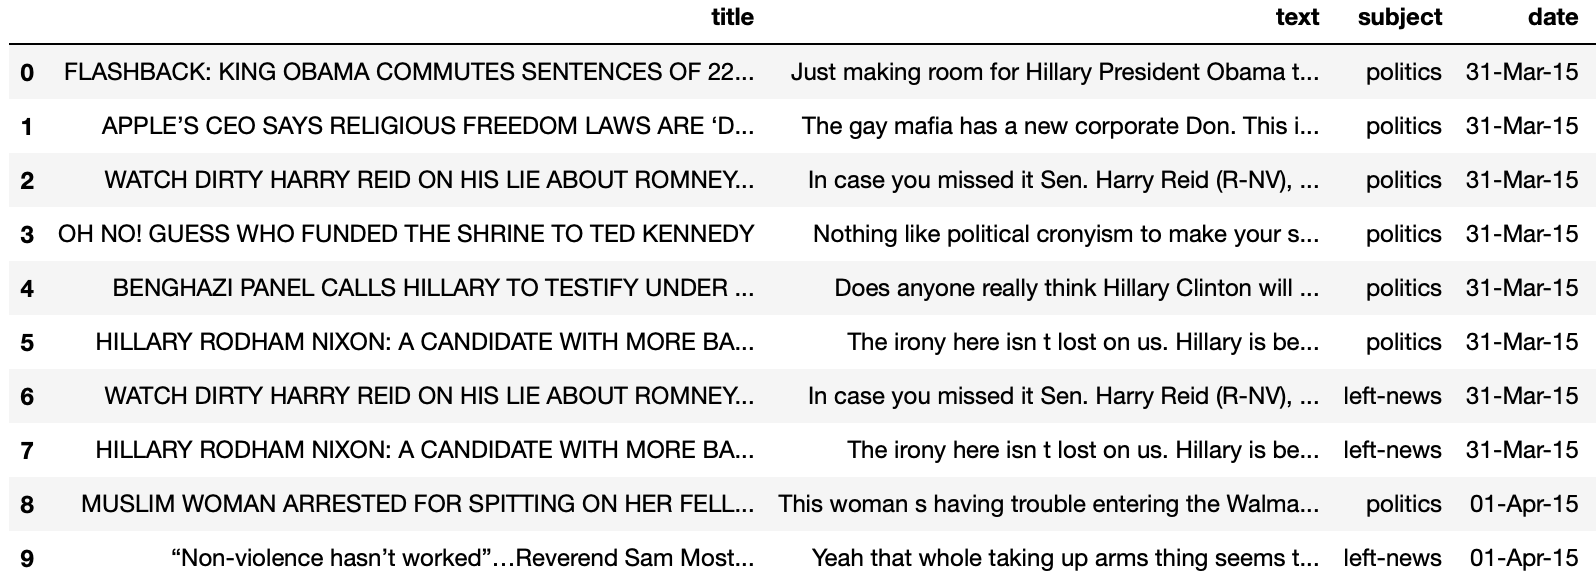
\includegraphics[scale=0.3]{dt_example.png}
\end{center}
\begin{center}
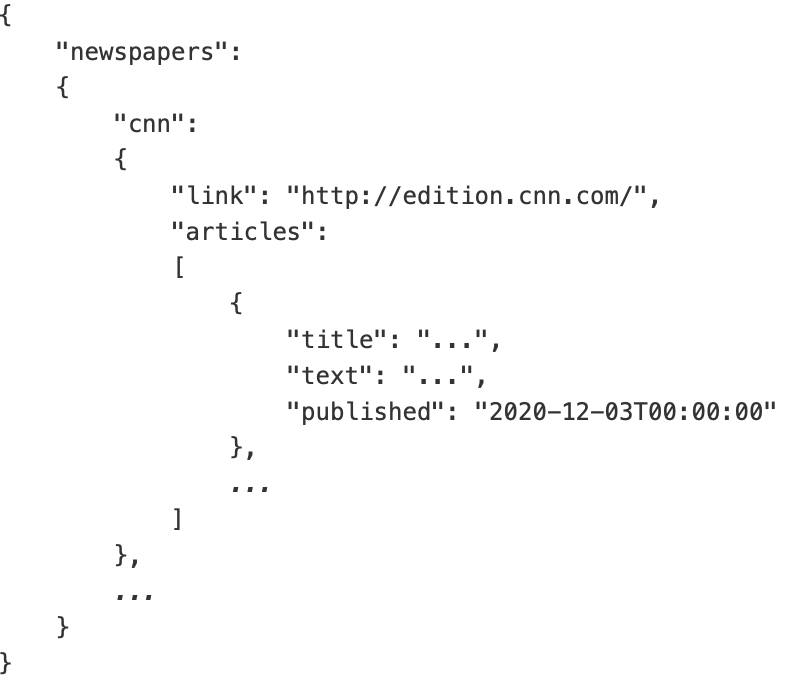
\includegraphics[scale=0.3]{scraped_example.png}
\end{center}
Our inspiration to utilize the Kaggle dataset in addition to a scraping approach came from a similar experiment in news classification conducted by Ria Gandhi \cite{Ria}, \cite{githubRia}. In addition, her approach in preprocessing of the data and her model selection were somewhat replicated in our project, albeit with many changes to implementation details and parameter tuning. The underlying goal of this experiment is to present the respective results from each model and compare their overall performance in classification. The results of our model training and the generated predictions will be presented analyzed in this report. Detailed graphs, confusion matrices, metrics measurement, and other results  for each of the classifiers as well as a report of accuracy, precision and recall metrics. 


%------------------------------------------------------------------------
\section{Methodology \& Experimental Results}
\small
The first step in our experiment was to carry out the preprocessing of the raw dataset. Preprocessing included steps such as the cleanup of the raw data from both Kaggle and scraped sources into the desired format, and then removing empty data cells, punctuation from each article's text formatting, and applying tokenization to each entry in the dataset using the Natural Language Processing Toolkit library. Tokenization allows for the extraction of all unique words from each article into a list of words as opposed to a single string object, while providing the option to exclude stop-words for words that are overtly present in the data or for words that the model should be agnostic to. Additionally in this process a dictionary of all the words in the dataset (i.e. vocabulary) was generated to define all the training features. For the purposes of this project, we chose to omit common words of the English language in addition to certain words that appear on every entry of the Kaggle dataset, notably "Reuters", since each "real" entry contained a reference to this well-known reputable news source.  In addition, we also applied a lemmatization to group together words that appear in several (inflected) forms. For instance, words that imply the same meaning such as "lying" and "lie" may be grouped together during this process.\par

After data cleanup and text tokenization, we vectorized the article entries by applying a TF-IDF Vectorizer to assign a normalized feature frequency mapping to our list of tokenized articles, which returns a sparse matrix that can be utilized for training all of the traditional machine learning models. The Convolutional Neural Network conversely was trained using a Count Vectorizer, which uses a non-normalized form of the frequency mapping (i.e. integer form instead of normalized floats) since this model classifies based on frequencies. This appeared to generate more desirable result for the Convolutional Neural Network during training and evaluation. After tokenization and generating the features to train the model with, the next step is to include the corresponding label for each article in the data, with the choice being "real" or "fake" and then combine all entries into a data frame. The last step of preprocessing was to split the data into testing and training samples, with a 30\% and 70\% split respectively.\par

The first model that was trained on the preprocessed data was the Logistic Regression classifier. We opted to tune the inverse regularization hyperparameter with 13 values in the logarithmic space ranging from 10\textsuperscript{-6} to 10\textsuperscript{6}. Hyperparameter tuning on this estimator was carried out by using the GridSearchCV method to determine the inverse regularization value that generated the best cross-validation core, which happened to be C=10. Choosing the optimal inverse regularization parameter yields a result with the most ideal trade-off between overfitting and accuracy.  In addition, we also calculated the training and testing accuracy for each hyperparameter, and plotted the result (as shown in the figure below). The small margin of difference between the test and training scores in the graph generally indicates that the Logistic Regression model has little overfitting, and that the test and training scores tend to converge which are both desirable outcomes.\par

After determining the best hyperparameter and training the model, the testing features were fed into the model to obtain a prediction of the corresponding labels, where "real" news is encoded as 0 and "fake" news is encoded as 1. We subsequently generated a graph of each of the training and testing scores as well as a confusion matrix (Figure~\ref{first_figure}) that helped us visualize predictions of the new articles. Please refer to the appendix to view side-by-side comparison of the distribution of fake vs. real news (Figure~\ref{piechart_1}). The model achieved a testing accuracy of 91.34\%, a mean squared error of 9.62\% and a precision of 90.78\% with a very low overfitting value of 0.009. \\

\begin{figure}[h]
   \begin{center}
        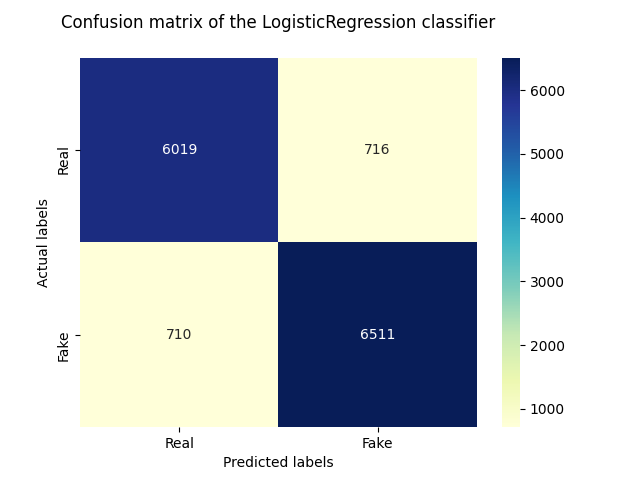
\includegraphics[width=\linewidth]{graphs/LR/confusion_matrix.png}
        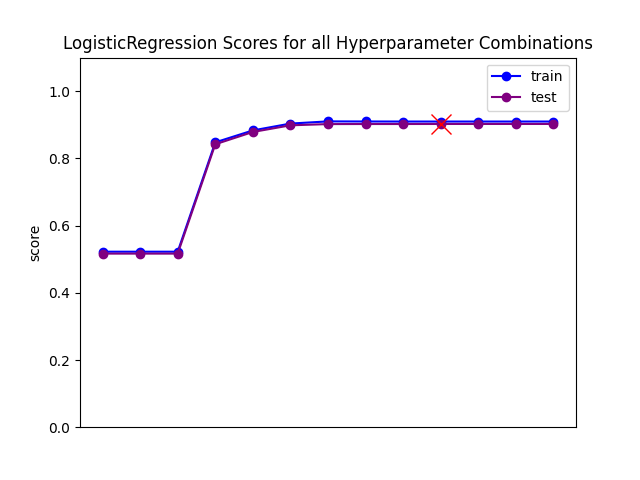
\includegraphics[width=\linewidth]{graphs/LR/scores_plot.png}
   \end{center}
        \vspace*{-5mm}
        \caption{\label{first_figure}}
\end{figure}
The Decision Tree classifier was the next model trained in the experiment. This model predicts the correct label for a particular article by learning simple decision rules inferred from the training data features. Only the max depth hyperparameter was used to train the model, whose value was likewise determined via cross-validation. The hyperparameter search was carried out with 50 values in the linear space ranging from 2 to 100. It was important to choose a wide enough range to ensure a better estimator, but without compromising computational performance which is the case with larger tree depths. The grid search yielded an optimal maximum tree depth parameter of 16. The model's overfitting value was also calculated based on the training and held-out scores over each hyperparameter, and similarly the result was graphed like with the Logistic Regression model. The result of the predictions performed by the Decision Tree classifier are depicted in the confusion matrix in Figure~\ref{Second_figure} in the appendix. The model achieved an accuracy of 86.14\%, a mean squared error of 13.86\% and a precision of 86.12\% with an overfitting value of 1.096.\par

The Random Forest classifier fits a number of Decision Tree classifiers on various sub-samples of a dataset, and generally yields better results than a single Decision Tree since it takes advantage of averaging. Predictive accuracy can be improved while also controlling over-fitting to a satisfying degree. Just like with the previous 2 models, a hyperparameter search using GridSearchCV was conducted to find the optimal maximum depth and number of estimators. The chosen parameters for the search were values in the linear space between 2 and 14 for max depth, and 10 values in the linear space between 2 and 20. It was important to perform the hyperparameter search in a reasonable range, in order to avoid excessively expensive computations and infeasible training situations given the time constraints of our experiment and size of our dataset. The hyperparameter search yielded the optimal tree depth as 14 and the optimal number of classifiers (decision trees) as 20. As with the previous models, a plot of the training and held-out scores and the prediction confusion matrix is depicted below, in addition to a plot displaying the feature importances for the top 25 words in Figure~\ref{Third_figure} in the appendix. Figure~\ref{piechart_3} shows the distribution of labels for the true and predicted. The model achieved an accuracy of 91.11\%, a mean squared error of 8.89\% and a precision of 91.25\% with an overfitting value of 1.42.\par

A Support Vector Machine model, which is a form of supervised learning, was then used to further help us in our quest for category prediction and classification. This model had an advantage of being memory efficient in the sense that it uses a subset of training points in the decision function called support vectors. In terms of the parameters used, we performed a hyperparameter search over 2 types of kernels, namely a Gaussian kernel of type 'rbf' and a linear kernel, with 5 values of C and gamma both ranging within the logarithmic space from 10\textsuperscript{-2} to 10\textsuperscript{2}. The best estimator with kernel='rbf', C=0.01, and gamma = 0.179 was returned by the grid search, and thus used in the predictions on the testing set. Refer to Figure~\ref{fourth_figure} in the appendix to visualize the result. The model achieved an accuracy of 60.73\%, a mean squared error of 39.27\% and a precision of 57.89\%.\par
Multinomial Naive Bayesian classifier was the next model chosen given its suitability for classification of discrete feature, such as the tokenized text in our preprocessed dataset. Like with the previous models, a grid search was performed over the hyperparameters alpha (discrete values between 0 and 50) and fit\_prior (true or false) to obtain the ideal estimator. The best estimator with fit\_prior=true and alpha=1.585 was returned by the grid search, and thus used in the predictions on the testing set. Refer to Figure~\ref{fifth_figure}. The model achieved an accuracy of 87.408\%, a mean squared error of 12.59\% and a precision of 90.01\% with an overfitting value of 0.022. \par

The last part of our experiment was to compare the classification of a supervised deep-learning model in contrast to more traditional machine learning models. We opted to use a Convolutional Neural Network, since it is well suited for text classification based on the frequency of occurrence for words. Since our preprocessing takes the frequencies of each into account, we felt that this model would be best suited to our data's structure. The implementation of this model was done with PyTorch relied heavily on the tutorial of Fernando Lopez \cite{Fernando}, \cite{githubFer}. The network is constructed of 11 layers – a dropout layer, an embedding layer, 4 convectional layers, 4 pooling layers, and 1 full-connected layer. \par
In terms of training parameters, we first opted to use a batch size of 108, 24 epochs, and a learning rate of 0.001. The losses generated during training and evaluation were diverging, since the learning rate was too large for the gradient descent, and was overshooting at each epoch. After tuning the learning rate to be a smaller value of 0.0001, the result was much better, with a solution that was converging with each epoch. Refer to the Figure~\ref{sixth_figure} below to visualize the results. In the appendix, plots depicting the accuracies over each epoch are shown Figure~\ref{seventh_figure}.
\begin{figure}[h]
   \begin{center}
       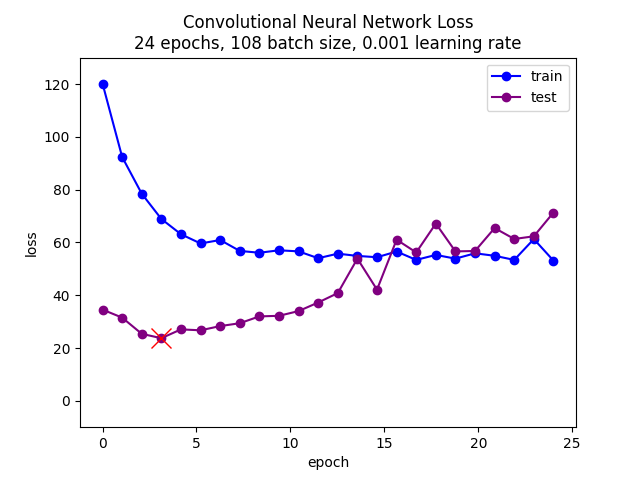
\includegraphics[width=\linewidth]{graphs/CNN/higher_learning_rate_loss_plot.png}
        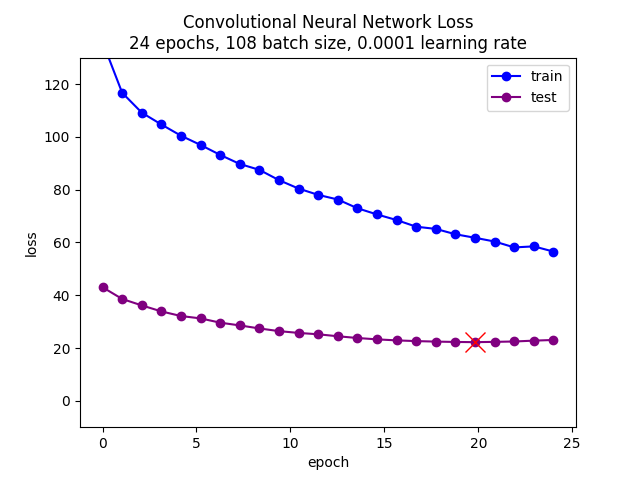
\includegraphics[width=\linewidth]{graphs/CNN/loss_plot.png}
   \end{center}
        \vspace*{-6mm}
        \caption{\label{sixth_figure}}
\end{figure}

%------------------------------------------------------------------------
\section{Conclusions}
\small
We have made the notable observation that the Logistic Regression classifier actually had the highest prediction accuracy at 91.34\% out of all the traditional models that were trained. The confusion matrix generated for this model demonstrates 6014 articles were correctly labelled as "real" and 6618 articles were correctly labelled as "fake". The degree of overfitting was also the lowest among the traditional models, with the absolute difference between the training and held-out scores being 0.009. We can conclude from the result that the Logistic Regression Classifier was the most accurate in classification among the traditional machine learning models used in the experiments. \par

Decision Tree Classifier follows the Bayesian model closely with a classification accuracy of 86.14\%. Its confusion matrix shows that the mode was able to correctly classify 5674 articles into the "Real" category and 6366 articles into the "Fake" category. The model was significantly slower to run than the Bayesian model at 1.2 minutes vs the 3 seconds the Bayesian model took to classify our data. It also had a much higher overfitting value at 1.096 and thus we can conclude that the Naive Bayesian model is better employed to solve our particular problem on the provided dataset.  \par

Logistic Regression was closely followed by the Random Forest classifier with an accuracy of 91.11\%. The confusion matrix generated for this classifier depicts quite similar results, with 6060 articles correctly labelled as "real" and 6675 articles correctly labelled as "fake". The model, however, had a significantly higher measured overfitting of 1.421 measured as the difference between the training and testing scores. Despite the marginal difference in accuracy, Logistic Regression remains at an advantage given its reduction in overfitting. \par

The least performant and perhaps the most disappointing of the classifiers, the Support Vector Machine was the only model that appeared to diverge, with a relatively high mean squared error. Additionally, the support vector machine classifier was the slowest to train, taking approximately 10.8 minutes to fully execute. The classification accuracy was also the lowest at 60.73\%. Despite poor performance, the model did not have much overfitting with a measured absolute score difference of only 0.142. A total of 1929 articles were correctly labelled as "real" compared to 6559 correctly labelled as "fake". The less than average performance is likely indicative of poorly chosen hyperparameters rather than it being an unsuitable estimator. Investigating into different sets of hyperparameters for the Support Vector Machine cross-validation could potentially lead to more accurate predictions in the future.\par

The Multinomial Naive Bayesian model ranked third in terms of performance with a classification accuracy of 87.41\%. Its confusion matrix demonstrates that the model was able to successfully classify 6011 articles as "real" and 6206 articles as "fake". One clear advantage of the Multinomial Naive Bayesian is its significantly faster run-time computation and its low measured overfitting of 0.022. The model only took approximately 4 seconds to run from start to finish, including the hyperparameter grid search that occupies the bulk of execution time. Even though the accuracy score is slightly lower than other models in the experiment, it has a clear advantage in the classification of larger datasets, and would likely scale better. \par

The Convolutional Neural Network seemed to yield quite interesting observations. Constructed with only 11 layers and 24 epochs already appeared to show promising results in terms of loss reduction and accuracy in both training and testing. The \par

It is important to note that every decision made in the process impacted the results, particularly the preprocessing and hyperparameter tuning. Correctly cleaning the raw data, tokenizing it with wisely chosen stopwords, using lemmatization, and applying the suitable vectorizer depending on the model all have contributed to the higher rates of accuracy. A good deal of time was spent investigating appropriate ranges of hyperparameters for each model to perform a grid search, which we conclude has yielded generally good results with the exception of the Support Vector Machine classifier.

The results of the model predictions in news article classification indicate that supervised machine learning models are capable of identifying fake news with a relatively high degree of accuracy. With a smaller dataset, we were able to generate prediction accuracies over 80\% for most of the models. Despite the general success of the majority of the experiments, it is difficult say with certainty if such models could be applied in a larger scale new classification system, given the limited nature of the dataset, potential bias in the data labelling, and the training methods used. Perhaps what is most promising are the initial results generated by the Convolutional Neural Network. With only a handful of layers, the model already had quite impressive results in terms of loss and accuracy for training and evaluation. Perhaps such a model could be extended with deeper layers and more data to help solve the crisis of online misinformation.

Note: please refer to the appendix to view more graphs depicting the classification results visually.

{\small
\raggedright
\bibliographystyle{ieeetr}
\bibliography{bibliography}
}

\newpage
\appendix
\onecolumn
%-------------------------------------------------------------------------
\section*{Appendix: Extra Results}\centering
\begin{table*}[!hb]\centering
   \begin{center}
   \begin{tabular}{|l|c|c|c|c|c|}
   \hline
    Classifier & Accuracy & Mean Squared Error & Precision & Recall & fscore\\
   \hline\hline
   Naive Bayes & 92.33\% & 27.7\% & 94.25\% & 90.87\% & 92.53\% \\
   Decision Tree & 99.22\% & 8.79\% & 99.03\% & 99.48\% & 99.26\% \\
   Random forest & 94.40\% & 23.60\% & 93.99\% & 95.41\% & 94.69\%\\
   Support Vector Machine & 90.90\% & 30.04\% & 91.24\% & 91.51\% & 91.38\% \\
   Logistic Regression & 99.08\% & 9.55\% & 99.14\% & 99.10\% & 99.13\% \\
   \hline
   \end{tabular}
   \end{center}
   \caption{Summary of Traditional ML Model Results\label{first_table}}
\end{table*}

\begin{figure}[h]
   \begin{center}
        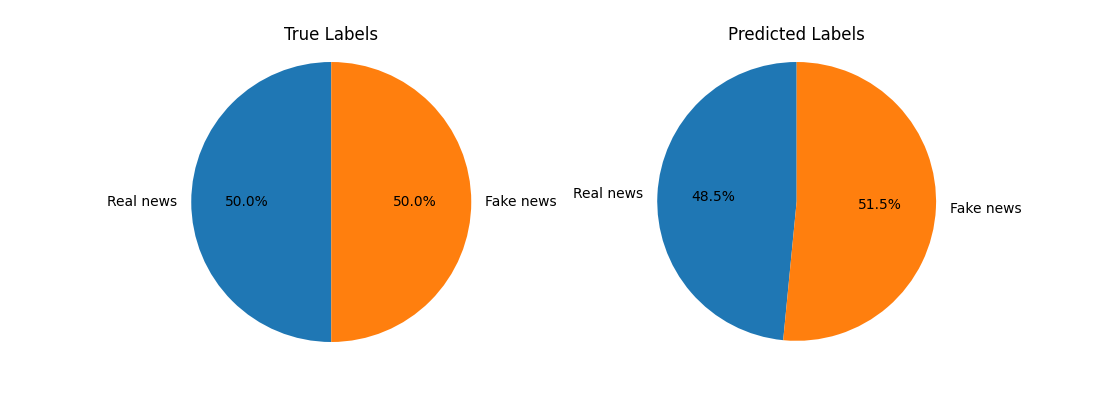
\includegraphics[scale=0.6]{graphs/LR/piechart.png}
   \end{center}
\vspace*{-5mm}
\caption{Logistic Regression results \label{piechart_1}}
\end{figure}

\begin{figure}[h]
   \begin{center}
        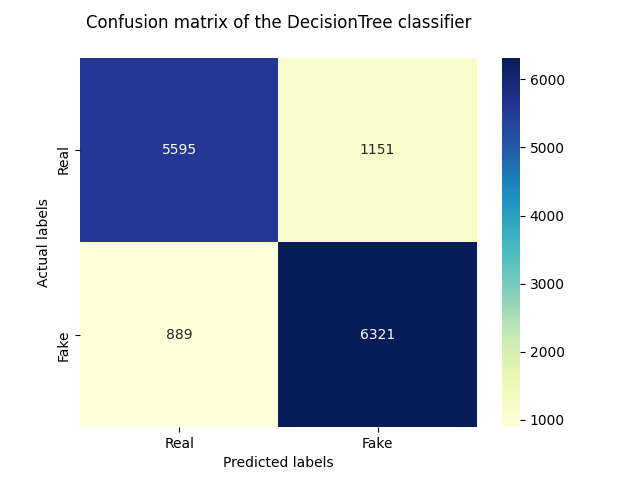
\includegraphics[scale=0.8]{graphs/DT/confusion_matrix.png}
        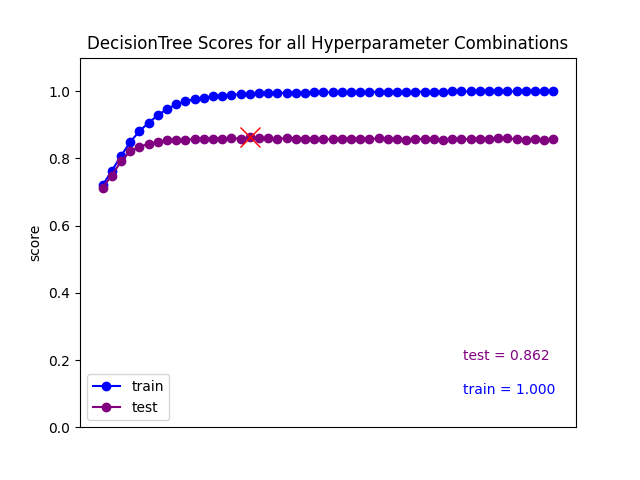
\includegraphics[scale=0.8]{graphs/DT/scores_plot.png}
        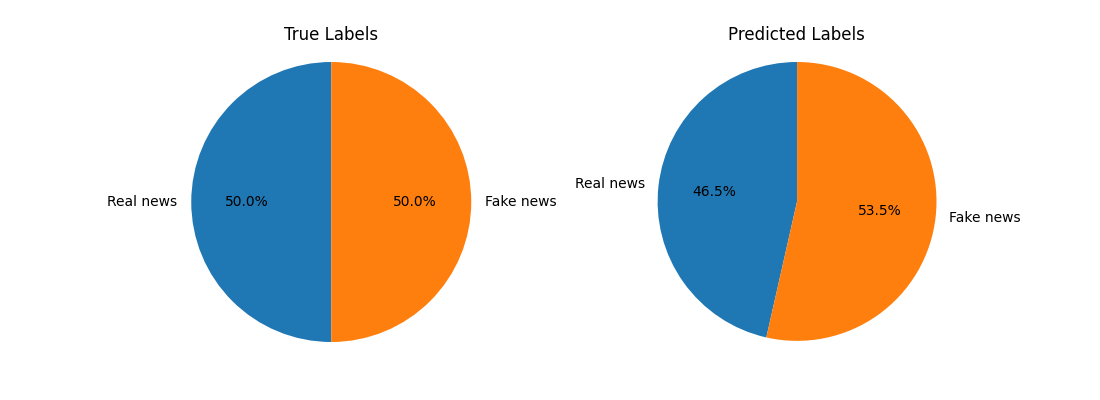
\includegraphics[scale=0.6]{graphs/DT/piechart.png}
   \end{center}
        \vspace*{-5mm}
        \caption{\label{Second_figure}}
\end{figure}

\begin{figure}[h]
   \begin{center}
        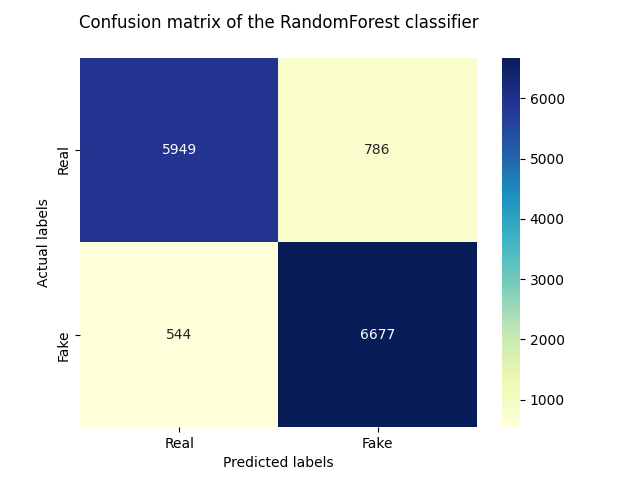
\includegraphics[scale=0.6]{graphs/RF/confusion_matrix.png}
        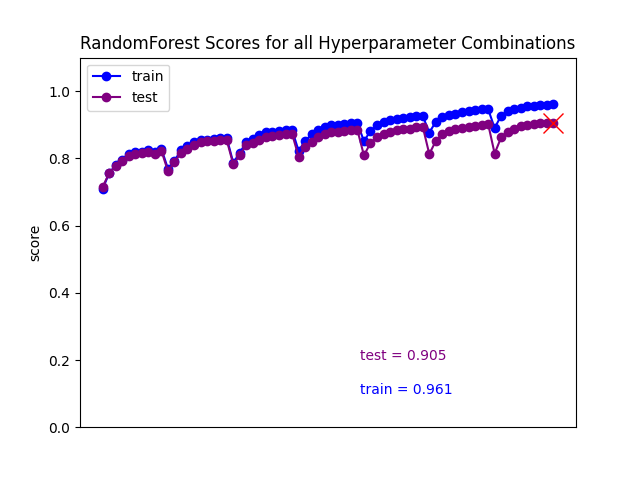
\includegraphics[scale=0.6]{graphs/RF/scores_plot.png}
        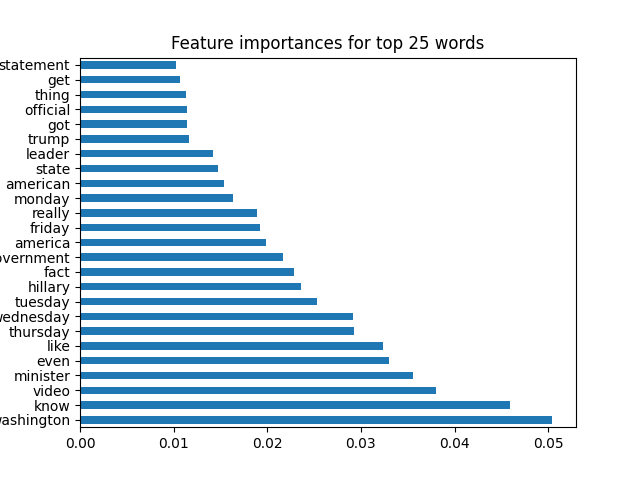
\includegraphics[scale=0.6]{graphs/RF/feature_importances.png}
   \end{center}
        \vspace*{-5mm}
        \caption{\label{Third_figure}}
\end{figure}

\begin{figure}[h]
   \begin{center}
        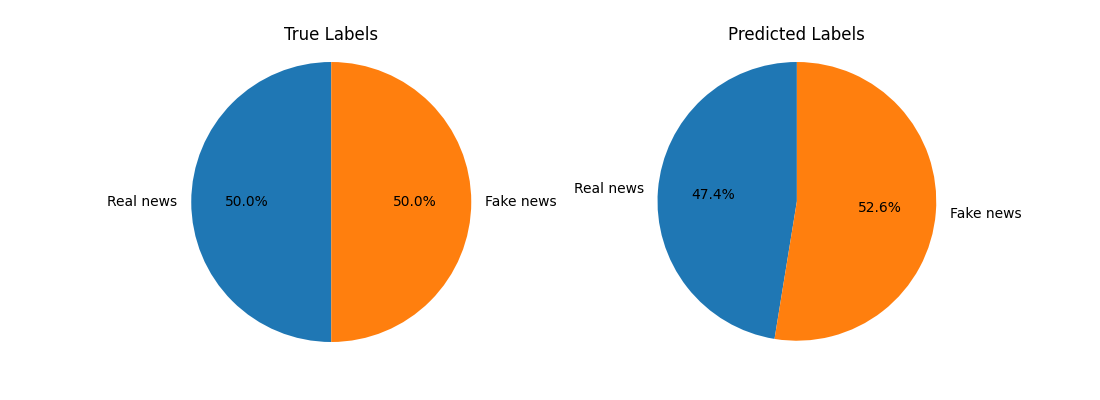
\includegraphics[scale=0.6]{graphs/RF/piechart.png}
   \end{center}
\vspace*{-5mm}
\caption{Random Forest results \label{piechart_3}}
\end{figure}

\begin{figure}[h]
   \begin{center}
        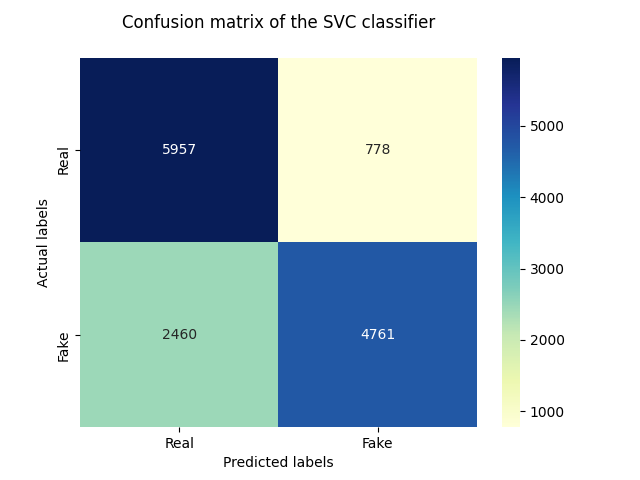
\includegraphics[scale=0.6]{graphs/SVC/confusion_matrix.png}
        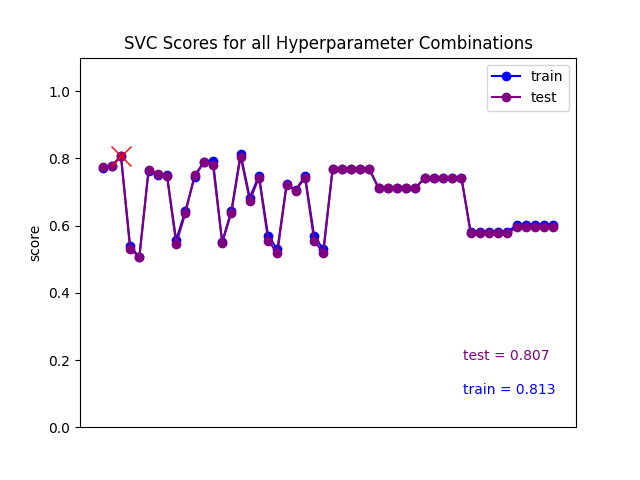
\includegraphics[scale=0.6]{graphs/SVC/scores_plot.png}
        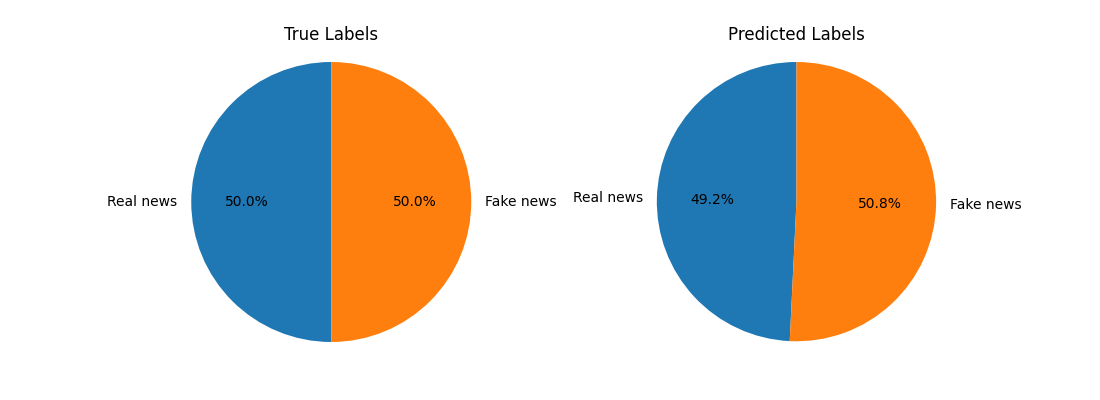
\includegraphics[scale=0.6]{graphs/SVC/piechart.png}
   \end{center}
        \vspace*{-5mm}
        \caption{\label{fourth_figure}}
\end{figure}

\begin{figure}[h]
   \begin{center}
        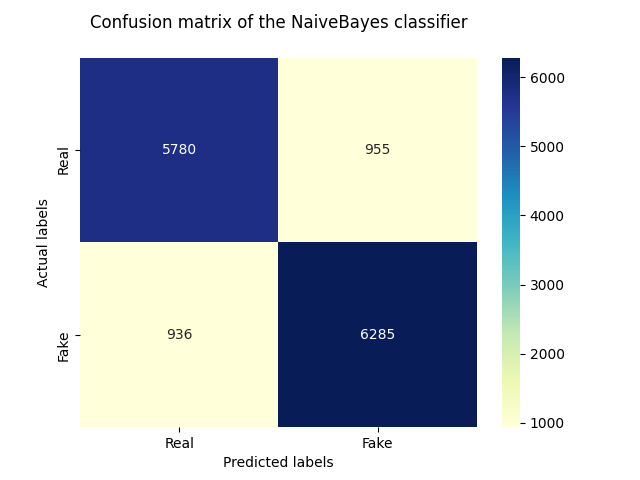
\includegraphics[scale=0.6]{graphs/NB/confusion_matrix.png}
        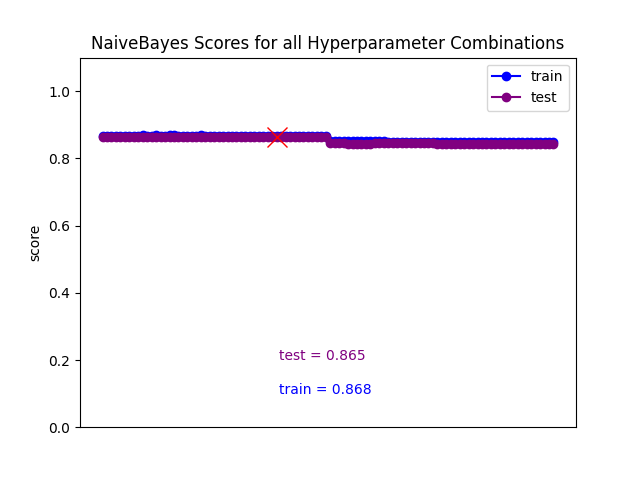
\includegraphics[scale=0.6]{graphs/NB/scores_plot.png}
        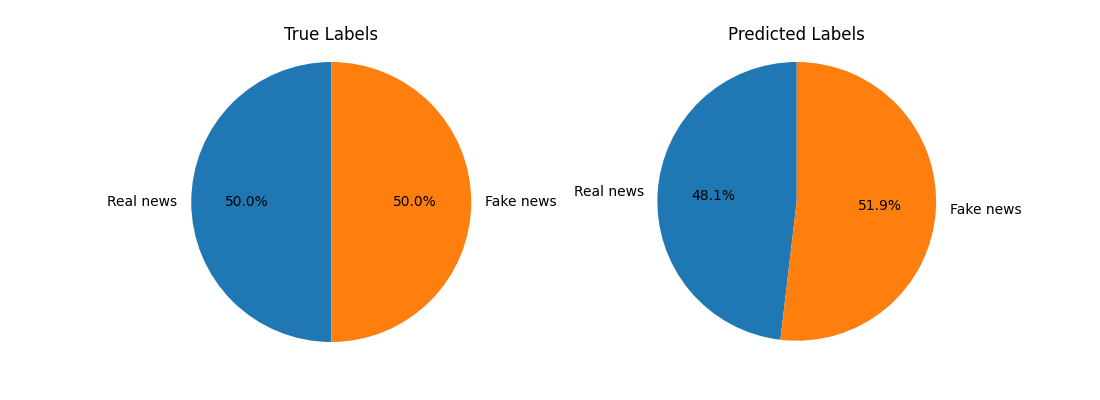
\includegraphics[scale=0.6]{graphs/NB/piechart.png}
   \end{center}
        \vspace*{-5mm}
        \caption{\label{fifth_figure}}
\end{figure}

\begin{figure}[h]
   \begin{center}
       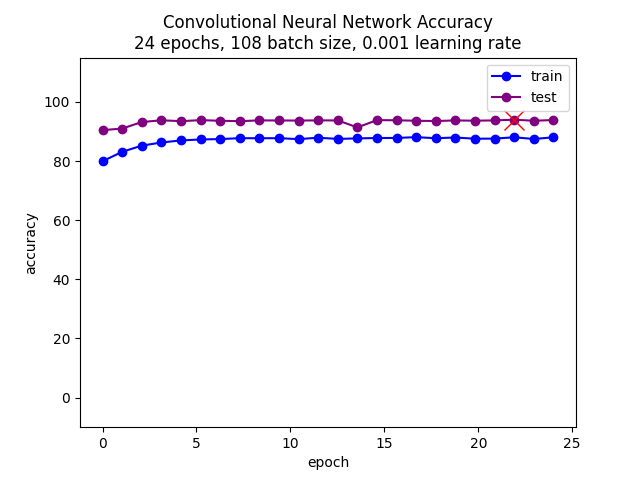
\includegraphics[scale=0.8]{graphs/CNN/higher_learning_rate_accuracies_plot.png}
        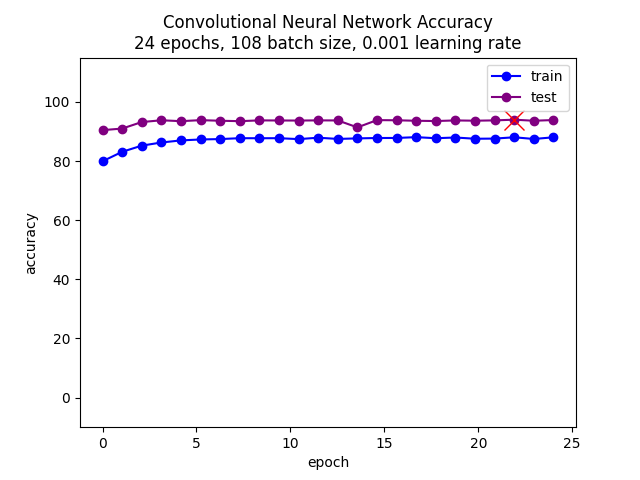
\includegraphics[scale=0.8]{graphs/CNN/accuracies_plot.png}
   \end{center}
        \vspace*{-5mm}
        \caption{\label{seventh_figure}}
\end{figure}

\end{document}
